\documentclass[11pt]{article}
\usepackage{amsmath, amssymb, amscd, amsthm, amsfonts}
\usepackage{graphicx}
\usepackage{hyperref}
\usepackage{algorithm}
\usepackage{algorithmic}
\usepackage{amsmath}
\usepackage{algorithm}
\usepackage[noend]{algpseudocode}
\usepackage{mathtools}
\usepackage{graphicx}
\usepackage{amsmath}
\usepackage[section]{placeins}
\usepackage{float}
\documentclass[sigconf,authordraft]{acmart}
\graphicspath{ {./images/} }


\newcommand\Myperm[2][^n]{\prescript{#1\mkern-2.5mu}{}P_{#2}}
\newcommand\Mycomb[2][^n]{\prescript{#1\mkern-0.5mu}{}C_{#2}}





 

\oddsidemargin 0pt
\evensidemargin 0pt
\marginparwidth 40pt
\marginparsep 10pt
\topmargin -20pt
\headsep 10pt
\textheight 8.7in
\textwidth 6.65in
\linespread{1.2}

\title{Home work 5}
\author{Vasanth Reddy Baddam}




%\author{Homework by Vasanth Reddy}
\date{04/20/2020}

\newtheorem{theorem}{Theorem}
\newtheorem{lemma}[theorem]{Lemma}
\newtheorem{conjecture}[theorem]{Conjecture}
\newcommand{\bigO}{\mathcal{O}}
\newcommand{\rr}{\mathbb{R}}

\newcommand{\al}{\alpha}
\DeclareMathOperator{\conv}{conv}
\DeclareMathOperator{\aff}{aff}
\def\lc{\left\lceil}   
\def\rc{\right\rceil}
\begin{document}

\maketitle
I pledge that this test/assignment has been completed in compliance with the Graduate Honor Code and
that I have neither given nor received any unauthorized aid on this test/assignment\\
\textbf{Name: } Vasanth Reddy Baddam\\
\textbf{Signature: } VB\\
\hline
\vspace{5mm}
\textbf{Q1}.\\
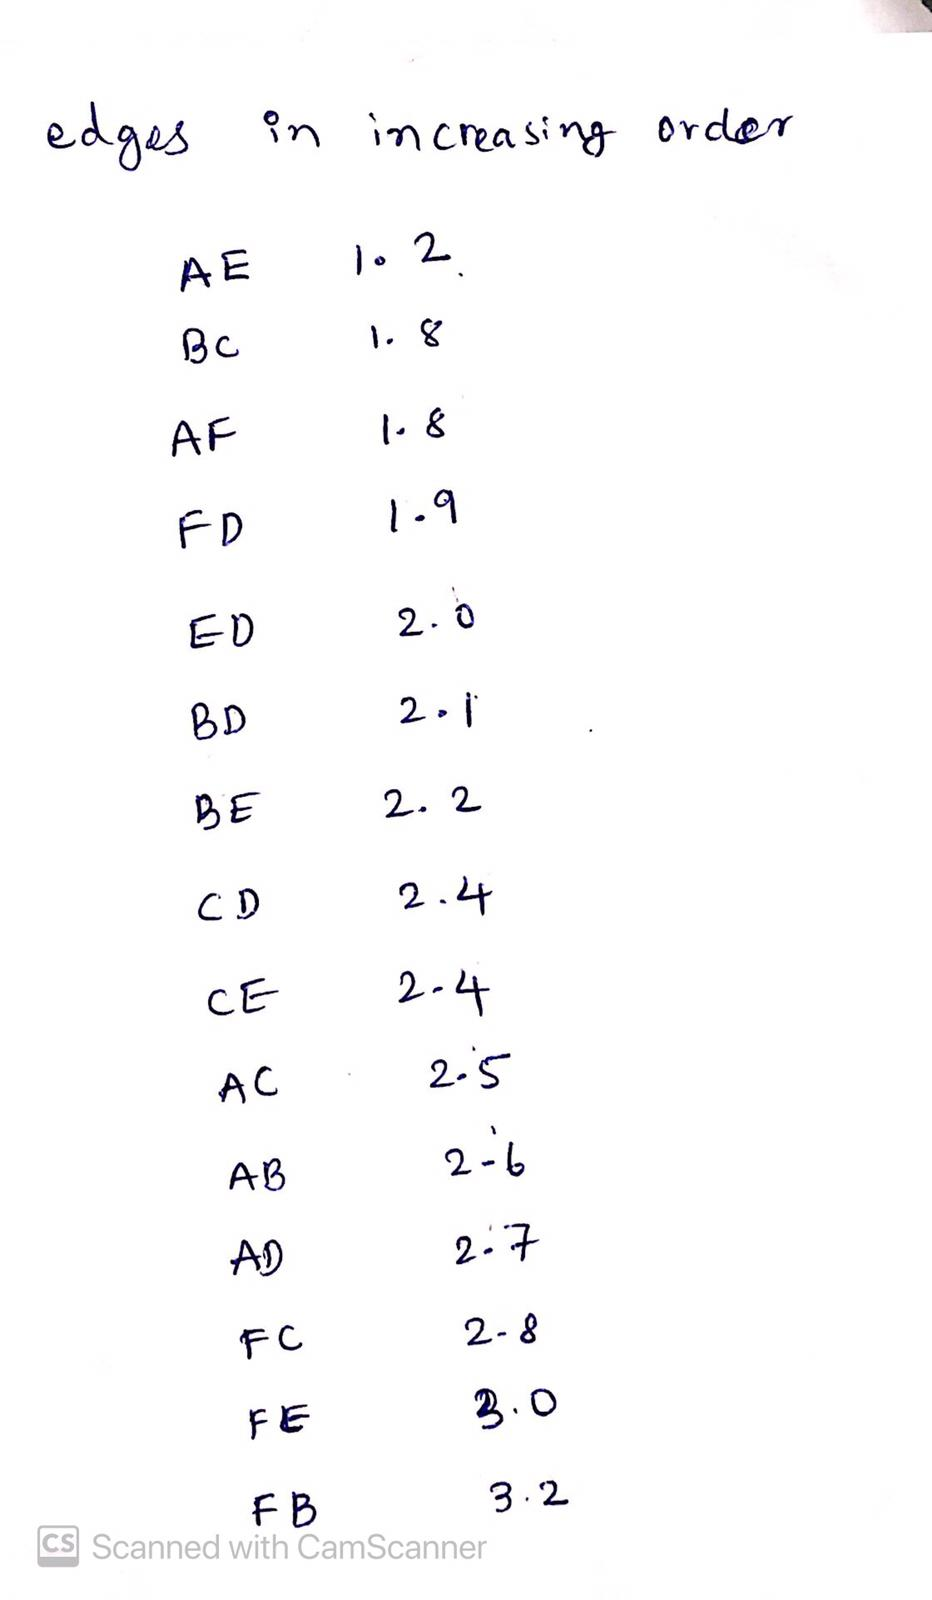
\includegraphics[scale = 0.2]{WhatsApp Image 2020-04-18 at 11.08.04 PM.jpeg}
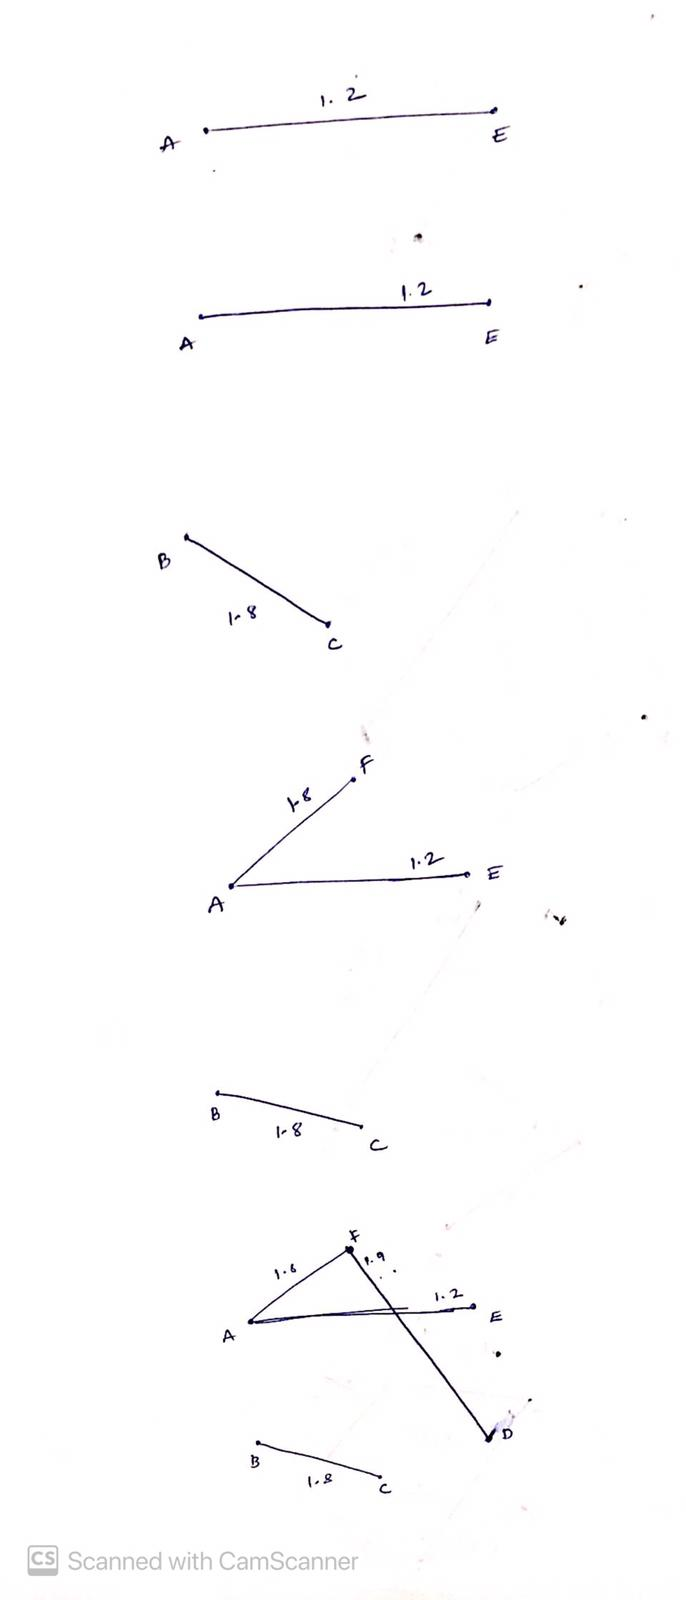
\includegraphics[scale = 0.2]{WhatsApp Image 2020-04-18 at 11.08.05 PM.jpeg}
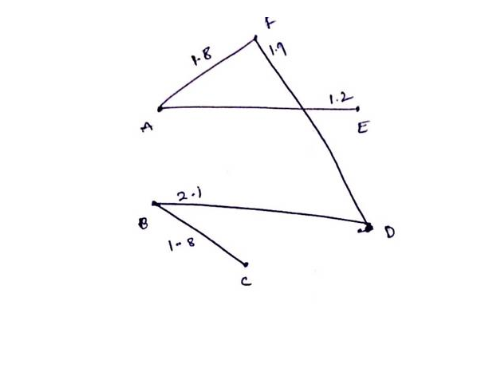
\includegraphics[scale=0.6]{wh.png}
\vspace{5mm}
\hline
\vspace{5mm}
\textbf{Q2}.\\
In Prim's Algorithm, we should select one vertex and start spreading the edges from that vertex. I selected vertex A and extended the edges from that vertex.
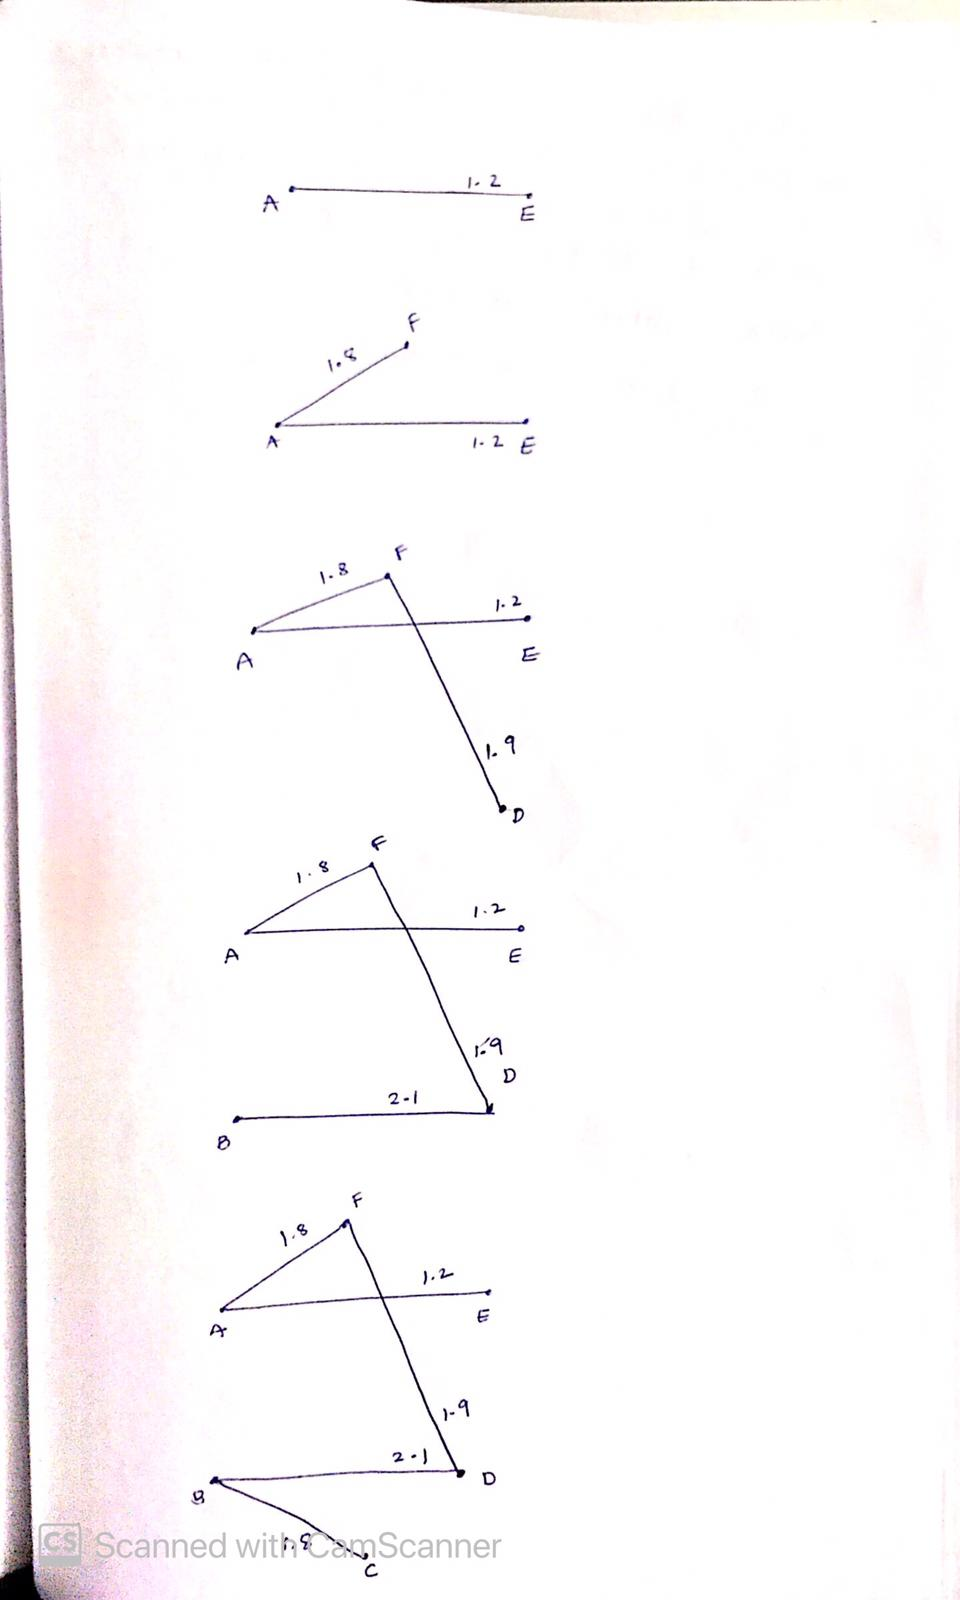
\includegraphics[scale=0.3]{WhatsApp Image 2020-04-19 at 8.59.23 PM.jpeg}
\vspace{5mm}
\hline
\vspace{5mm}
\textbf{Q3}.\\
If a graph is given $G = (V, E)$ is a directed graph then the transpose of that such graph would be obtained by reversing the direction of arrows we get $G^T = (V, E^T)$. In adjacent matrix case, Adjacency matrix for graph $G$ is given by $A = [a_{ij}]$. Adjacency matrix for $G^T$ is given by $A^T = [a^{T}_{ij}]$, where $a^{T}_{ij} = a_{ji}$. So, we need to find the transpose of the matrix $A$\\

\begin{algorithm}
\caption{Transpose of Adjacency matrix}\label{euclid}
\begin{algorithmic}
\Procedure{\textsc{Matrix Transpose}(\textit{G, $G^T$})}{}
\State e = number of edges
\For{$i$ in range of e}
\For{$j$ in range of e}
\State $G^T[i][j] = G[j][i]$
\EndFor
\EndFor
\end{algorithmic}
\end{algorithm}

As the algorithm is running it's all vertices twice. Time complexity of the above algorithm is \bigO($e^2$) , i.e \bigO($V^2$)\\

\begin{algorithm}
\caption{Transpose of Adjacency List}\label{euclid}
\begin{algorithmic}
\Procedure{\textsc{Adjacency List Transpose}(\textit{G})}{}
\For{$u$ in range of V[G]}
\For{element $v \in $Adj[u]}
\State Insert $u$ in front of Adj[v]
\EndFor
\EndFor
\end{algorithmic}
\end{algorithm}

Time complexity is \bigO(V+E)

\vspace{5mm}
\hline
\vspace{5mm}
\textbf{Q4.}\\
 \begin{table}[htp]
\begin{tabular}{|l|r|r|r|}
\toprule
edge($i,j$) &  White &  Gray &  Black \\
\midrule
White    &       T,B,F,C &  B,C &     C \\
Gray &       T,F &  T,F,B &     T,F,C  \\
Black       &        &  B &     T,F,B,C \\
\bottomrule
\end{tabular}
\caption {Directed Graph}
\end{table} 

 \begin{table}[htp]
\begin{tabular}{|l|r|r|r|}
\toprule
edge($i,j$) &  White &  Gray &  Black \\
\midrule
White    &       T,B &  T,B &      \\
Gray &       T,B &  T,B &     T,B  \\
Black       &        &  T,B &     T,B \\
\bottomrule
\end{tabular}
\caption {UnDirected Graph}
\end{table} 

\vspace{20mm}
\hline
\vspace{20mm}
\textbf{Q5.}\\
After running the Slow-all-pairs-shortest-path algorithm, we get the following output : \\\\ 
\vspace*{3ex}L$^{(1)}$ (Initial matrix)\\
$\begin{bmatrix}
0 & \infty & \infty & \infty & -1 & \infty\\
1 & 0 & \infty & 2 & \infty & \infty\\
\infty & 2 & 0 & \infty & \infty & -8\\
-4 & \infty & \infty & 0 & 3 & \infty\\
\infty & 7 & \infty & \infty & 0 & \infty\\
\infty & 5 & 10 & \infty & \infty & 0
\end{bmatrix}$\\\\\\
\vspace*{3ex}L$^{(2)}$ (m = 2)\\
$\begin{bmatrix}
0 & 6 & \infty & \infty & -1 & \infty\\
-2 & 0 & \infty & 2 & 0 & \infty\\
3 & -3 & 0 & 4 & \infty & -8\\
-4 & 10 & \infty & 0 & -5 & \infty\\
8 & 7 & \infty & 9 & 0 & \infty\\
6 & 5 & 10 & 7 & \infty & 0
\end{bmatrix}$\\\\\\
\vspace*{3ex}L$^{(3)}$ (m = 3)\\
$\begin{bmatrix}
0 & 6 & \infty & 8 & -1 & \infty\\
-2 & 0 & \infty & 2 & -3 & \infty\\
-2 & -3 & 0 & -1 & 2 & -8\\
-4 & 2 & \infty & 0 & -5 & \infty\\
5 & 7 & \infty & 9 & 0 & \infty\\
3 & 5 & 10 & 7 & 5 & 0
\end{bmatrix}$\\\\\\
\vspace*{3ex}L$^{(4)}$ (m = 4)\\
$\begin{bmatrix}
0 & 6 & \infty & 8 & -1 & \infty\\
-2 & 0 & \infty & 2 & -3 & \infty\\
-5 & -3 & 0 & -1 & -3 & -8\\
-4 & 2 & \infty & 0 & -5 & \infty\\
5 & 7 & \infty & 9 & 0 & \infty\\
3 & 5 & 10 & 7 & 2 & 0
\end{bmatrix}$\\\\\\
\vspace*{3ex}L$^{(5)}$ (m = 5)\\
$\begin{bmatrix}
0 & 6 & \infty & 8 & -1 & \infty\\
-2 & 0 & \infty & 2 & -3 & \infty\\
-5 & -3 & 0 & -1 & -6 & -8\\
-4 & 2 & \infty & 0 & -5 & \infty\\
5 & 7 & \infty & 9 & 0 & \infty\\
3 & 5 & 10 & 7 & 2 & 0
\end{bmatrix}$\\\\\\
\vspace{5mm}
\hline
\vspace{5mm}
\textbf{Q6.}\\
After running the Flyod-Warshall algorithm, we get the following output : \\\\ 
\vspace*{3ex}D$^{(0)}$ (Initial matrix)\\
$\begin{bmatrix}
0 & \infty & \infty & \infty & -1 & \infty\\
1 & 0 & \infty & 2 & \infty & \infty\\
\infty & 2 & 0 & \infty & \infty & -8\\
-4 & \infty & \infty & 0 & 3 & \infty\\
\infty & 7 & \infty & \infty & 0 & \infty\\
\infty & 5 & 10 & \infty & \infty & 0
\end{bmatrix}$\\\\\\
\vspace*{3ex}D$^{(1)}$ (k = 1)\\
$\begin{bmatrix}
0 & \infty & \infty & \infty & -1 & \infty\\
1 & 0 & \infty & 2 & 0 & \infty\\
\infty & 2 & 0 & \infty & \infty & -8\\
-4 & \infty & \infty & 0 & -5 & \infty\\
\infty & 7 & \infty & \infty & 0 & \infty\\
\infty & 5 & 10 & \infty & \infty & 0
\end{bmatrix}$\\\\\\
\vspace*{3ex}D$^{(2)}$ (k = 2)\\
$\begin{bmatrix}
0 & \infty & \infty & \infty & -1 & \infty\\
1 & 0 & \infty & 2 & 0 & \infty\\
3 & 2 & 0 & 4 & 2 & -8\\
-4 & \infty & \infty & 0 & -5 & \infty\\
8 & 7 & \infty & 9 & 0 & \infty\\
6 & 5 & 10 & 7 & 5 & 0
\end{bmatrix}$\\\\\\
\vspace*{3ex}D$^{(3)}$ (k = 3)\\
$\begin{bmatrix}
0 & \infty & \infty & \infty & -1 & \infty\\
1 & 0 & \infty & 2 & 0 & \infty\\
3 & 2 & 0 & 4 & 2 & -8\\
-4 & \infty & \infty & 0 & -5 & \infty\\
8 & 7 & \infty & 9 & 0 & \infty\\
6 & 5 & 10 & 7 & 5 & 0
\end{bmatrix}$\\\\\\
\vspace*{3ex}D$^{(4)}$ (k = 4)\\
$\begin{bmatrix}
0 & \infty & \infty & \infty & -1 & \infty\\
-2 & 0 & \infty & 2 & -3 & \infty\\
0 & 2 & 0 & 4 & -1 & -8\\
-4 & \infty & \infty & 0 & -5 & \infty\\
5 & 7 & \infty & 9 & 0 & \infty\\
3 & 5 & 10 & 7 & 2 & 0
\end{bmatrix}$\\\\\\
\vspace*{3ex}D$^{(5)}$ (k = 5)\\
$\begin{bmatrix}
0 & 6 & \infty & 8 & -1 & \infty\\
-2 & 0 & \infty & 2 & -3 & \infty\\
0 & 2 & 0 & 4 & -1 & -8\\
-4 & 2 & \infty & 0 & -5 & \infty\\
5 & 7 & \infty & 9 & 0 & \infty\\
3 & 5 & 10 & 7 & 2 & 0
\end{bmatrix}$\\\\\\
\vspace*{3ex}D$^{(6)}$ (k = 6)\\
$\begin{bmatrix}
0 & 6 & \infty & 8 & -1 & \infty\\
-2 & 0 & \infty & 2 & -3 & \infty\\
-5 & -3 & 0 & -1 & -6 & -8\\
-4 & 2 & \infty & 0 & -5 & \infty\\
5 & 7 & \infty & 9 & 0 & \infty\\
3 & 5 & 10 & 7 & 2 & 0
\end{bmatrix}$\\\\\\

\end{document}

